\documentclass[11pt,letterpaper]{article}

\usepackage[letterpaper,margin=0.8in,nohead]{geometry}

\usepackage[colorlinks]{hyperref}
\usepackage{url}
\usepackage{breakurl}

\hypersetup{
	colorlinks,
	linkcolor={red},
	citecolor={red},
	urlcolor={blue}
}

\usepackage{verbatim}
\usepackage{fancyvrb}
\usepackage{scrextend}
\usepackage{enumitem}
\usepackage{url}
\usepackage{subcaption}

\usepackage{filecontents}
%\usepackage{natbib}
%\nobibliography*

\usepackage{caption}
\usepackage{graphicx}

\usepackage{changepage}   % for the adjustwidth environment

\newenvironment{answer}{\em \color{blue} \begin{adjustwidth}{1cm}{1cm}}{\end{adjustwidth}}

% math
\usepackage{amsthm,amsmath}
\usepackage{amsfonts}

\newcommand{\mc}[1]{\mathcal{#1}}	% Mechanisms / Algorithms
\newcommand{\rv}[1]{\mathbf{#1}}    % Random variable

\newcommand{\pr}[1]{\mathrm{Pr}\{#1\}} % Probability

\newtheorem{corollary}{\bf Corollary}%[theorem]
\newtheorem{lemma}{\bf Lemma}%[theorem]
\newtheorem{definition}{\bf Definition}%[section]

\newtheorem{observation}{\bf Observation}%[theorem]



% load cleveref last!
\usepackage[capitalise]{cleveref}

\crefname{observation}{Observation}{Observations}


\begin{document}
	
	\title{EN3240: Embedded Systems Engineering \\Assignment 6 --- Validation/Verification \& Security}
	
	%% This is an individual assignment!!
	%% TODO: put your name and index number here!
	\author{Name: Thalagala B. P. \\ Index No: 180631J}
	
	\maketitle
	
	\begin{center}
		\color{red}\bf This is an individual assignment! \\ Due Date: 7 October 2022 by 11.59 PM
	\end{center}
	
	\section*{Instructions}
	%
	
	Please read the instructions and questions carefully. Write your answers directly in the space provided. Compile the tex document and submit the resulting PDF. This is an individual assignment. You are not allowed to take or give any help in completing this assignment.
	
	%%%%%%%%%%%%%%%%%%%%%%%%%%%%%%%%%
	%%%%%%%%%%%%%%%%%%%%%%%%%%%%%%%%%
	\newpage
	
	\section*{Problem 1 (1 Point)}
	
	How many input patterns (tests) are required (minimum) to verify a 3-input OR gate completely when only binary inputs are allowed (each input can be 0 or 1)? List the inputs and expected outputs.
	
	%% TODO: add answer here
	
	\vspace{50mm}
	
	%%%%%%%%%%%%%%%%%%%%%
	%%%%%%%%%%%%%%%%%%%%%
	%%%%%%%%%%%%%%%%%%%%%
	
	\section*{Problem 2 (2 Points)}
	
	How many input patterns (tests) are required (minimum) to verify a 3-input OR gate completely when only ternary inputs are allowed (each input can be 0 or 1 or x;  x implies unknown which can be 0 or 1)? List the inputs.
	
	%% TODO: add answer here
	
	\vspace{40mm}
	
	%%%%%%%%%%%%%%%%%%%%%
	%%%%%%%%%%%%%%%%%%%%%
	%%%%%%%%%%%%%%%%%%%%%
	
	\section*{Problem 3 (2 Points)}
	
	There are two types of processor simulation techniques - functional and cycle-accurate. Given an input assembly program, the functional simulation produces the correct output but does not provide cycle-by-cycle  details. On  the  other  hand,  the  pipelined  simulation  provides  a cycle-by-cycle  simulation  of  the pipeline  to  eventually  produce  the  final  result. Which one  is  faster  in  terms  of  performance  (simulation time) and why? Why do people use the slower one, then?
	
	%% TODO: add answer here
	
	%%%%%%%%%%%%%%%%%%%%%
	%%%%%%%%%%%%%%%%%%%%%
	%%%%%%%%%%%%%%%%%%%%%
	
	\newpage
	\section*{Problem 4 (2 Points)}
	
	There are only two ways of combining compression and encryption: 
	
	\begin{itemize}
		\item CASE I: compression followed by encryption.
		\item CASE II: encryption followed by compression.
	\end{itemize}
	
	Please  indicate  which  is beneficial for both  code  size  reduction  and  security  improvement.  Please explain why the other one is not suitable.
	
	%% TODO: add answer here
	
	\vspace{25mm}
	
	%%%%%%%%%%%%%%%%%%%%%
	%%%%%%%%%%%%%%%%%%%%%
	%%%%%%%%%%%%%%%%%%%%%
	
	\section*{Problem 5 (8 Points)}
	
	\begin{enumerate}
		\item Download the shadow.hex file from the ``assignment6-resources'' folder. This file has been encrypted using RC4 encryption. 40 bits hexadecimal key: \textcolor{magenta}{6D 69 74 72 65}. Decrypt the file using any available decryption tool (e.g., cryptool). Add a screenshot of the decrypted shadow.hex file content.
		
		\begin{figure}[h]
			\centering
			\fbox{
				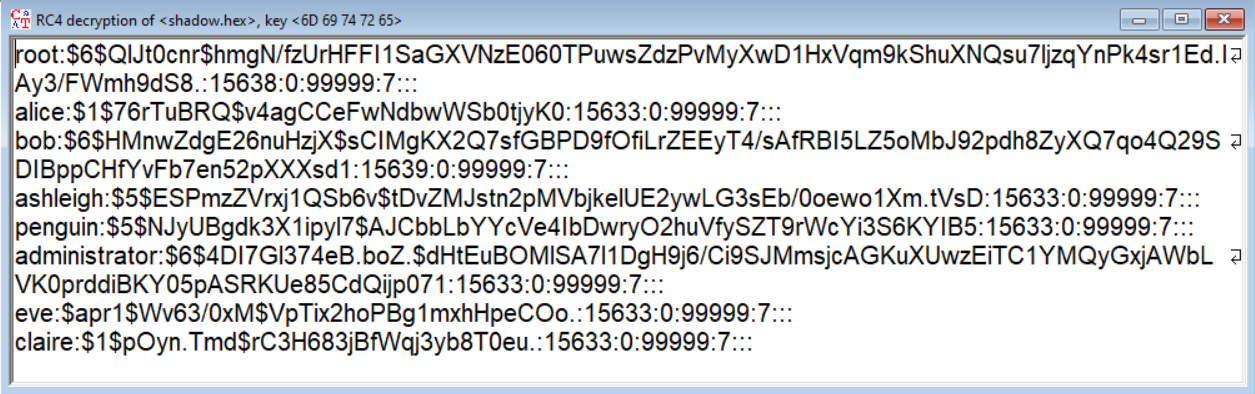
\includegraphics[width=0.85\columnwidth]{problem5/decryptshadow.PNG}
			}
		\caption{Content of the decrypted ``{\tt shadow.hex}'' file}
		\end{figure}
		
		
		\vspace{25mm}
		
		%%%%%%%%%%%%%%%%%%%%%
		%%%%%%%%%%%%%%%%%%%%%
		%%%%%%%%%%%%%%%%%%%%%
		
		\item Run ``John the Ripper'' password cracking utility to crack the passwords in the decrypted shadow file with the help of the dictionary ``rockyou.txt''(\href{https://uniofmora-my.sharepoint.com/:t:/g/personal/scharles_uom_lk/EQvMHge3CrZNpeE7WGXpapoBslFMMcgHih0teepNIwDVIg?e=9aEjJd}{Link}). What is the command you used to crack the passwords in the shadow file? 
		
		%% TODO: add answer here
		
		\vspace{10mm}
		
		%%%%%%%%%%%%%%%%%%%%%
		%%%%%%%%%%%%%%%%%%%%%
		%%%%%%%%%%%%%%%%%%%%%
		
		\item Add a screenshot of all the cracked passwords.
		
		%% TODO: add answer here
		
		\vspace{35mm}
		
		%%%%%%%%%%%%%%%%%%%%%
		%%%%%%%%%%%%%%%%%%%%%
		%%%%%%%%%%%%%%%%%%%%%
		
		\item Provide recommendations to enhance the strength of the passwords.
		
		%% TODO: add answer here
		
		%%%%%%%%%%%%%%%%%%%%%
		%%%%%%%%%%%%%%%%%%%%%
		%%%%%%%%%%%%%%%%%%%%%
		
		\clearpage
		
	\end{enumerate}    
	
	%%%%%%%%%%%%%%%%%%%%%%%%%%%%%%%%%
	%%%%%%%%%%%%%%%%%%%%%%%%%%%%%%%%%    
\end{document}
